\subsection{Leerlaufspannung und Innenwiderstand}
\label{sec:LeerRi}
Die genommenen Messwerte werden im ersten Schritt, mit der notierten Skala,
in die tatsächlichen Werte umgerechnet. Ein Strich in den Tabellen oder eine
unterschiedliche Farbe in den Plots zeigt eine Veränderung der Skala des Amperemeters an.
Im folgenden bezeichnen
\begin{align*}
  U_{0,X} \: &\text{die Leerlaufspannung und} \\
      R_\text{i,X} \: &\text{den Innenwiderstand der Spannungsquelle X.}
\end{align*}

\subsubsection{Monozelle}
\label{sec:monozelle}
Die lineare Regression, nach
\begin{equation*}
      U_\text{k} = \symbf{I} R_\text{i} + U_0,
\end{equation*}
ergibt
\begin{align}
      R_\text{i,m} &= \SI{5.64(14)}{\ohm}
      \label{eqn:rimono} \\
      U_{0,\symup{m}} &= \SI{1.423(006)}{\volt}.
      \label{eqn:u0mono}
\end{align}
Im Plot \ref{fig:mono} sind die Werte aus \ref{tab:mono} und die Ausgleichsgerade zu sehen.
\begin{figure}
      \centering
      \includegraphics[width=\textwidth]{build/mono.pdf}
      \caption{Messwerte und Ausgleichsgerade bzgl der Monozelle.}
      \label{fig:mono}
\end{figure}
\begin{table}
      \centering
      \caption{Messwerte der Monozelle.}
      \label{tab:mono}
      \begin{tabular}{S[table-format=1.4] S[table-format=1.2] | S[table-format=1.4] S[table-format=1.2]}
            \toprule
            \multicolumn{2}{c|}{Messwerte-1} & \multicolumn{2}{c}{Messwerte-2} \\
            \hline
            $\symbf{I} \: [\si{\milli\ampere}]$ & $U_\text{k} \: [\si{\volt}]$ & $\symbf{I} \: [\si{\milli\ampere}]$ & $U_\text{k} \: [\si{\volt}]$ \\
            \midrule
            0.0200 & 1.32 & 0,0300 & 1,25 \\
            0.0215 & 1.31 & 0,0340 & 1,23 \\
            0.0220 & 1.30 & 0,0365 & 1,21 \\
            0.0235 & 1.30 & 0,0410 & 1,19 \\
            0.0265 & 1.29 & 0,0440 & 1,17 \\
            0.0265 & 1.28 & 0,0495 & 1,14 \\
            0.0267 & 1.27 & 0,0545 & 1,10 \\
            0.0265 & 1.26 & 0,0625 & 1,06 \\
                   &      & 0,0700 & 1,02 \\
                   &      &  0,0902& 0,94 \\
            \bottomrule
      \end{tabular}
\end{table}

\newpage

\subsubsection{Rechteckspannung}
\label{sec:rechteck}
Die tatsächlichen Stromstärken für die $\SI{3}{\milli\ampere}$-Skala berechnen sich nach
\begin{align}
      \frac{M}{30} &= \frac{\symbf{I}}{\SI{3e-3}{\ampere}}
      \intertext{- $M$ sind die gemessenen Werte -}
      \symbf{I} &= \frac{\SI{3e-3}{\ampere}}{30} M \\
      \symbf{I} &= M \cdot 10^{-4} \si{\ampere}.
\end{align}
Für die Skalierung von $\SI{10}{\milli\ampere}$ ergibt sich ebenfalls $\SI{1e-4}{\ampere}$
als Umrechnungsfaktor.

\noindent Die lineare Regression,
\begin{align}
      m &= \frac{\overline{xy} - \overline{x} \cdot \overline{y}}{\overline{\left(x^2\right)} - \left(\overline{x}\right)^2} \\
      b &= \overline{y} - m \overline{x},
\end{align}
für Gleichung \eqref{eqn:linreg}, ergibt, nach Skalierung des Amperemeters getrennt,
die Werte aus Tabelle \ref{tab:linregrechteck}.
\begin{table}
      \centering
      \caption{Werte der linearen Regression.}
      \label{tab:linregrechteck}
      \begin{tabular}{c| S[table-format=2.1] @{${}\pm{}$} S[table-format=1.1] S[table-format=1.3] @{${}\pm{}$} S[table-format=1.3]}
            \toprule
            {Messwerte} & \multicolumn{2}{c}{$R_\text{i,r} \: [\si{\ohm}]$} & \multicolumn{2}{c}{$U_{0,\symup{r}} \: [\si{\volt}]$} \\
            \midrule
            1 & 59,0 & 2,3 & 0,701 & 0,006 \\
            2 & 58,1 & 0,6 & 0,718 & 0,003 \\
      \end{tabular}
\end{table}
\newpage
Wie im Plot \ref{fig:rechteck} zu sehen, verlaufen die Ausgleichsgeraden
nahezu parallel.
Mit dem Mittelwert
\begin{align}
      \overline{R_\text{i,r}} &= \frac{1}{2} \sum_{m=0}^{2} R_\text{i,r,m} = \SI{58.4}{\ohm}
      \intertext{und der Standardabweichung}
      \symup{σ_\text{i,r}} &= \sqrt{\overline{R_\text{i,r}^2} - {\overline{R_\text{i,r}}}^2} = \sqrt{\SI{3410,65}{\ohm\squared} - \SI{4310,56}{\ohm\squared}} = \SI{0,3}{\ohm}.
      \intertext{folgt}
      R_\text{i,r} &= \SI{58.4(3)}{\ohm}.
\end{align}
\begin{figure}
      \centering
      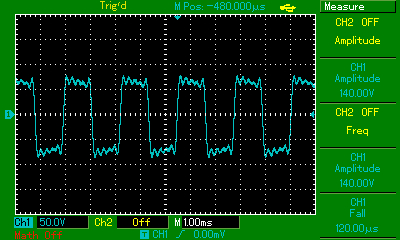
\includegraphics[width=\textwidth]{build/rechteck.pdf}
      \caption{Messwerte und Ausgleichsgeraden für die Rechteckspannung.}
      \label{fig:rechteck}
\end{figure}
\begin{table}
      \centering
      \caption{Messwerte der Rechteckspannung.}
      \label{tab:rechteck}
      \begin{tabular}{ S[table-format=1.2] S[table-format=1.3] | S[table-format=1.2] S[table-format=1.3]}
            \toprule
            \multicolumn{2}{c|}{Messwerte-1} & \multicolumn{2}{c}{Messwerte-2} \\
            \hline
            $\symbf{I} \: [\si{\milli\ampere}]$ & $U_\text{k} \: [\si{\volt}]$ & $\symbf{I} \: [\si{\milli\ampere}]$ & $U_\text{k} \: [\si{\volt}]$ \\
            \midrule
            2.15 & 0.572 & 3,70 & 0,502 \\
            2.19 & 0.571 & 3,88 & 0,492 \\
            2.30 & 0.569 & 4,10 & 0,481 \\
            2.39 & 0.561 & 4,39 & 0,463 \\
            2.48 & 0.555 & 4,60 & 0,450 \\
            2.60 & 0.550 & 4,90 & 0,433 \\
            2.71 & 0.540 & 5,40 & 0,408 \\
            2.86 & 0.532 & 6,00 & 0,370 \\
            2.99 & 0.525 & 6,61 & 0,332 \\
            \bottomrule
      \end{tabular}
\end{table}

\newpage

\subsubsection{Sinusspannung}
\label{sec:sinus}
Die lineare Regression, für \eqref{eqn:linreg} ergibt:

\begin{table}
      \centering
      \caption{Werte der linearen Regression.}
      \label{tab:linregsinus}
      \begin{tabular}{c | S[table-format=3.0] @{${}\pm{}$} S[table-format=2.0] S[table-format=1.3] @{${}\pm{}$} S[table-format=1.3]}
            \toprule
            {Messwerte} & \multicolumn{2}{c}{$R_\text{i,s} \: [\si{\ohm}]$} & \multicolumn{2}{c}{$U_{0,\symup{s}} \: [\si{\volt}]$} \\
            \midrule
            1 & 587 & 16 & 0,999 & 0,003 \\
            2 & 700 & 80 & 1,05  & 0,04 \\
      \end{tabular}
\end{table}
Aufgrund des Plots \ref{fig:sinus} wählen wir $R_\text{i,s} = R_\text{i,s1}$,
da die erste Messwertgruppe in nur sehr geringer Abweichung zu der entsprechenden Geraden liegt
und die zweite Messwertgruppe nicht ähnlich gut zu der zweiten Geraden liegt,
aber dennoch ausreichend gut für die erste Gerade.
\begin{figure}
      \centering
      \includegraphics[width=\textwidth]{build/sinus.pdf}
      \caption{Messwerte und Ausgleichsgeraden für die Sinusspannung.}
      \label{fig:sinus}
\end{figure}
\begin{table}
      \centering
      \caption{Messwerte der Sinusspannung.}
      \label{tab:sinus}
      \begin{tabular}{ S[table-format=1.3] S[table-format=1.3] | S[table-format=1.3] S[table-format=1.3]}
            \toprule
            \multicolumn{2}{c|}{Messwerte-1} & \multicolumn{2}{c}{Messwerte-2} \\
            \hline
            $\symbf{I} \: [\si{\milli\ampere}]$ & $U_\text{k} \: [\si{\volt}]$ & $\symbf{I} \: [\si{\milli\ampere}]$ & $U_\text{k} \: [\si{\volt}]$ \\
            \midrule
            0.154 & 0.910 & 0,380 & 0,802 \\
            0.156 & 0.909 & 0,425 & 0,731 \\
            0.160 & 0.905 & 0,480 & 0,720 \\
            0.166 & 0.900 & 0,550 & 0,666 \\
            0.171 & 0.899 & 0,638 & 0,609 \\
            0.171 & 0.894 &  &  \\
            0.186 & 0.889 &  &  \\
            0.194 & 0.885 &  &  \\
            0.204 & 0.882 &  &  \\
            0.223 & 0.871 &  &  \\
            0.236 & 0.862 &  &  \\
            0.258 & 0.849 &  &  \\
            0.282 & 0.830 &  &  \\
            \bottomrule
      \end{tabular}
\end{table}

\newpage
